\documentclass[a4paper, man, floatsintext]{apa6}
\usepackage{lmodern}
\usepackage{amssymb,amsmath}
\usepackage{ifxetex,ifluatex}
\usepackage{fixltx2e} % provides \textsubscript
\ifnum 0\ifxetex 1\fi\ifluatex 1\fi=0 % if pdftex
  \usepackage[T1]{fontenc}
  \usepackage[utf8]{inputenc}
\else % if luatex or xelatex
  \ifxetex
    \usepackage{mathspec}
  \else
    \usepackage{fontspec}
  \fi
  \defaultfontfeatures{Ligatures=TeX,Scale=MatchLowercase}
\fi
% use upquote if available, for straight quotes in verbatim environments
\IfFileExists{upquote.sty}{\usepackage{upquote}}{}
% use microtype if available
\IfFileExists{microtype.sty}{%
\usepackage{microtype}
\UseMicrotypeSet[protrusion]{basicmath} % disable protrusion for tt fonts
}{}
\usepackage{hyperref}
\hypersetup{unicode=true,
            pdfauthor={Jana B. Jarecki},
            pdfborder={0 0 0},
            breaklinks=true}
\urlstyle{same}  % don't use monospace font for urls
\usepackage{graphicx,grffile}
\makeatletter
\def\maxwidth{\ifdim\Gin@nat@width>\linewidth\linewidth\else\Gin@nat@width\fi}
\def\maxheight{\ifdim\Gin@nat@height>\textheight\textheight\else\Gin@nat@height\fi}
\makeatother
% Scale images if necessary, so that they will not overflow the page
% margins by default, and it is still possible to overwrite the defaults
% using explicit options in \includegraphics[width, height, ...]{}
\setkeys{Gin}{width=\maxwidth,height=\maxheight,keepaspectratio}
\IfFileExists{parskip.sty}{%
\usepackage{parskip}
}{% else
\setlength{\parindent}{0pt}
\setlength{\parskip}{6pt plus 2pt minus 1pt}
}
\setlength{\emergencystretch}{3em}  % prevent overfull lines
\providecommand{\tightlist}{%
  \setlength{\itemsep}{0pt}\setlength{\parskip}{0pt}}
\setcounter{secnumdepth}{0}
% Redefines (sub)paragraphs to behave more like sections
\ifx\paragraph\undefined\else
\let\oldparagraph\paragraph
\renewcommand{\paragraph}[1]{\oldparagraph{#1}\mbox{}}
\fi
\ifx\subparagraph\undefined\else
\let\oldsubparagraph\subparagraph
\renewcommand{\subparagraph}[1]{\oldsubparagraph{#1}\mbox{}}
\fi

%%% Use protect on footnotes to avoid problems with footnotes in titles
\let\rmarkdownfootnote\footnote%
\def\footnote{\protect\rmarkdownfootnote}

%%% Change title format to be more compact
\usepackage{titling}

% Create subtitle command for use in maketitle
\providecommand{\subtitle}[1]{
  \posttitle{
    \begin{center}\large#1\end{center}
    }
}

\setlength{\droptitle}{-2em}

  \title{}
    \pretitle{\vspace{\droptitle}}
  \posttitle{}
    \author{Jana B. Jarecki}
    \preauthor{\centering\large\emph}
  \postauthor{\par}
      \predate{\centering\large\emph}
  \postdate{\par}
    \date{01 November, 2019}

\usepackage{natbib} \usepackage{threeparttable} \usepackage{booktabs}
\shorttitle{test} \usepackage{setspace}
\AtBeginEnvironment{tabular}{\singlespacing} \usepackage{times}
\usepackage{changes} \definechangesauthor[name={JJ}, color=orange]{jj}
\usepackage{upgreek} \AtBeginDocument{\let\maketitle\relax}

\begin{document}

\subsection{Evaluations of Gambles by Condition and Sample Size}

Table \ref{tab:means_study2} displays participants' mean and median
evaluations per gamble in the experience and description conditions by
sample-size. The results resemble the findings of Study 1, namely that
larger sample sizes do not lead to systematic changes in mean
evaluations. Evaluations were best predicted by a linear model including
expected value as random factor and gamble type as fixed factor gamble
(additional fixed factor sample size: \(BF\textsubscript{01} = 285\);
additional interaction between sample size and gamble type:
\(BF\textsubscript{01} > 1,000\)).

\begin{table}[tbp]

\begin{center}
\begin{threeparttable}

\caption{\label{tab:means_study2}Valuations of Gambles in Study 1}

\begin{tabular}{lccccrr}
\toprule
Condition & Sample size category & Effective sample size & \textit{Med} & \textit{M} & D--E & D--E:$BF\textsubscript{10}$\\
\midrule
Gamble ID 1 &  &  &  &  &  & \\
\ \ \ E & xs & 5 & 5.15 & 6.29 & -0.85 & 11\\
\ \ \ E & s & 10 & 5.00 & 6.39 & -0.96 & 354\\
\ \ \ E & m & 15 & 5.95 & 6.38 & -0.95 & 72\\
\ \ \ E & l & 30 & 6.00 & 6.53 & -1.09 & 174\\
\ \ \ D & -- & -- & 4.00 & 5.43 & -- & --\\
Gamble ID 2 &  &  &  &  &  & \\
\ \ \ E & xs & 6 & 4.00 & 4.55 & -0.24 & 0\\
\ \ \ E & s & 12 & 4.00 & 4.72 & -0.41 & 1\\
\ \ \ E & m & 18 & 5.00 & 4.88 & -0.57 & 4\\
\ \ \ E & l & 36 & 4.95 & 4.78 & -0.47 & 3\\
\ \ \ D & -- & -- & 3.35 & 4.31 & -- & --\\
Gamble ID 3 &  &  &  &  &  & \\
\ \ \ E & xs & 7 & 8.95 & 10.65 & -1.41 & 6\\
\ \ \ E & s & 14 & 10.00 & 10.26 & -1.01 & 1\\
\ \ \ E & m & 21 & 9.70 & 10.37 & -1.12 & 2\\
\ \ \ E & l & 42 & 10.00 & 11.18 & -1.93 & 235\\
\ \ \ D & -- & -- & 6.00 & 9.25 & -- & --\\
Gamble ID 4 &  &  &  &  &  & \\
\ \ \ E & xs & 5 & 3.30 & 2.91 & 0.29 & 13\\
\ \ \ E & s & 10 & 3.20 & 2.94 & 0.26 & 27\\
\ \ \ E & m & 15 & 3.20 & 3.02 & 0.19 & 2\\
\ \ \ E & l & 30 & 3.20 & 3.09 & 0.11 & 0\\
\ \ \ D & -- & -- & 3.50 & 3.20 & -- & --\\
Gamble ID 5 &  &  &  &  &  & \\
\ \ \ E & xs & 6 & 2.00 & 1.82 & 0.10 & 1\\
\ \ \ E & s & 12 & 2.00 & 1.85 & 0.07 & 0\\
\ \ \ E & m & 18 & 2.00 & 1.85 & 0.06 & 0\\
\ \ \ E & l & 36 & 2.10 & 1.95 & -0.03 & 0\\
\ \ \ D & -- & -- & 2.00 & 1.92 & -- & --\\
Gamble ID 6 &  &  &  &  &  & \\
\ \ \ E & xs & 7 & 4.00 & 3.68 & 0.16 & 1\\
\ \ \ E & s & 14 & 4.10 & 3.78 & 0.07 & 0\\
\ \ \ E & m & 21 & 4.15 & 3.85 & -0.01 & 0\\
\ \ \ E & l & 42 & 4.20 & 3.90 & -0.05 & 0\\
\ \ \ D & -- & -- & 4.10 & 3.84 & -- & --\\
\bottomrule
\addlinespace
\end{tabular}

\begin{tablenotes}[para]
\normalsize{\textit{Note.} \textit{M} = mean, \textit{Med} = median, D--E = difference between mean description-based valuations and experience-based valuations, $BF\textsubscript{10}$ = Bayes Factor quantifying the evidence for a linear model $\mathrm{M}\textsubscript{1}$ predicting that valuations differ between description and experience over a linear model $\mathrm{M}\textsubscript{0}$ predicting no such differences; both models models contain a by-participant random effect. Gambles IDs 1, 2, and 3 are \$-bets; Gamble IDs 4, 5, and 6 are p-bets.}
\end{tablenotes}

\end{threeparttable}
\end{center}

\end{table}

\subsection{Cognitive modeling of experience-based evaluations}
\added[id=jj]{The modeling procedure followed the procedure in Study~1.}

\subsubsection{Modeling Results}
\added[id=jj]{The next section presents the quantitative cognitive model fit, the qualitative model fit, and lastly the effects of sample size given the cognitive strategies.}

\textit{Quantitative Model Fit.} The Bayesian value updating model
described the majority of the participants best (23 of 40; 57\%). The
relative frequency model described 17 participants best (42\%); the
baseline model described no participants best. Figure
\ref{fig:study2_model_weights} shows the evidence strength for the
models by participant. The models' mean Bayesian information criterion
across all participants equaled BIC\textsubscript{BVU}\(= -96\),
BIC\textsubscript{RF}\(= -91\), and BIC\textsubscript{BASE}\(= -17\)
(lower values indicate better fit).

\begin{figure}[htb]

{\centering 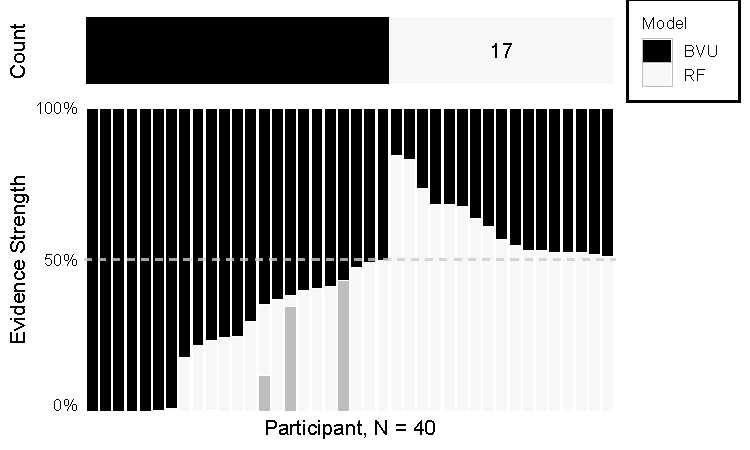
\includegraphics{../figures/study2_model_weights-1} 

}

\caption{Evidence for the models for individual participants. \textit{RF}$=$ relative frequency model, \textit{BVU}$=$ Bayesian value updating model, \textit{BASE}$=$ Baseline model.}\label{fig:study2_model_weights}
\end{figure}

\added[id=jj]{
The estimated parameter of the winning models are shown in Table \ref{tab:study2_parameter}. The mean power utility exponent $\alpha$ is relatively similar for participants classified as using a Bayesian value updating strategy ($M_{\alpha}= 2.19$) compared to those using a relative frequency strategy ($M_{\alpha}=2.15$), $M = 0.04$ 95\% HDI $[-1.08$, $1.16]$, $\mathrm{BF}_{\textrm{01}} = 3.21$. Like in Study 1, the participants using the Bayesian strategy had a loss prior, on avarage; they believed that gains occur with 45\% (gain prior $\theta_G = 0.91$; zero-outcome prior $\theta_0 = 1.09$). Again, the learning rate parameter $\delta$ shows liberal learning ($M_{\delta}=2.27$).
}

\begin{table}[tbp]

\begin{center}
\begin{threeparttable}

\caption{\label{tab:study2_parameter}Parameter Estimates of Winning Models, \textit{M (SD)}}

\begin{tabular}{lcccc}
\toprule
Winning Model & $\alpha$ & $\delta$ & $\theta_G$ & $\sigma$\\
\midrule
BVU (\textit{n}$=$23) & 2.19 (2.35) & 2.27 (3.39) & 0.91 (0.79) & 0.23 (0.22)\\
RF (\textit{n}$=$17) & 2.15 (1.45) & -- & -- & 0.15 (0.04)\\
\bottomrule
\addlinespace
\end{tabular}

\begin{tablenotes}[para]
\normalsize{\textit{Note.} \textit{BVU}$=$ Bayesian value updating model, \textit{RF}$=$ relative frequency model. Parameters denote: $\alpha=$ power utility exponent, $\theta_G$ gain prior, $\sigma$ standard deviation.}
\end{tablenotes}

\end{threeparttable}
\end{center}

\end{table}

\textit{Qualitative Model Fit.}
\added[id=jj]{Figure \ref{fig:ind_fits1} illustrates the qualitative model fit by plotting the predictions of the best-fitting models against the observed evaluations. The models generally describe the data well (mean $r\textsubscript{pred,obs} = 0.70$). However, some participants data are qualitatively not well described by the winning models (participants number 02, 07, 14, 27, with $r\textsubscript{pred,obs} < 0.40$). For one of these cases, the relative frequency model was favored, for the remaining three cases the Bayesian value updating model was favored.\footnote{Note, however, that participant number 7 evaluated all gambles with zero, which indicates inattentiveness or not comprehending the task.}}

\begin{figure}[htb]

{\centering 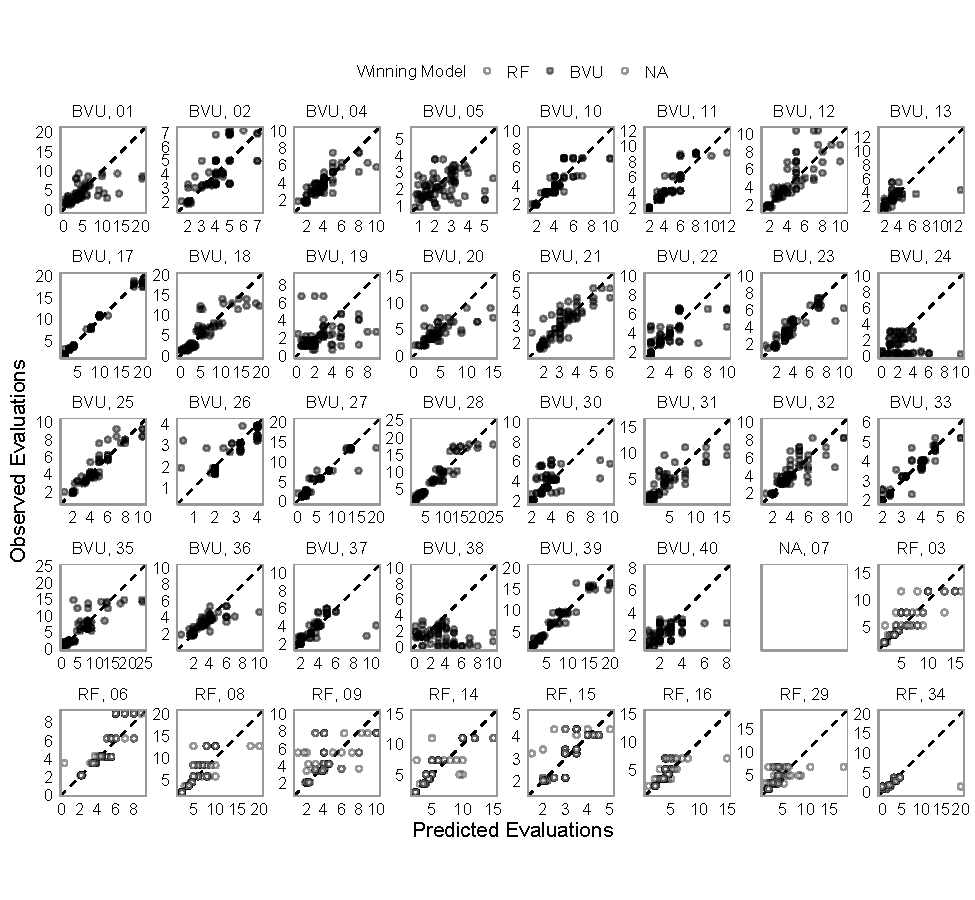
\includegraphics{../figures/ind_fits1-1} 

}

\caption{Predicted evaluations from the best-fitting models plotted against the observed evaluations (by participant). \textit{BVU}$=$ Bayesian value updating model, \textit{RF}$=$ relative frequency model, \textit{BASE}$=$baseline model.}\label{fig:ind_fits1}
\end{figure}

\added[id=jj]{The cognitive modeling results thus show greater heterogeneity in Study 2 (compared to Study 1), slightly more than half the participants could be described by a Bayesian strategy, the remaining participants followed a relative-frequency strategy. The higher prevalence of the relative frequency strategy in Study 2 can be explained considering that Study 2 initially withheld the information about the magnitude of the gain outcomes as opposed to Study 1, where participants received outcome information. If participants learn not only probabilities but also outcomes, the task might require more cognitive effort and this might take attention away from prior beliefs.}

\emph{The effect of sample size given cognitive strategies.}
\added[id=jj]{We qualitatively investigated how sample size affects the evaluations of relative-frequency-type and Bayesian-type learners. The Bayesian model predicts that sample size changes the evaluations in interaction with the prior beliefs. Participants with a gain prior should decrease the evaluations of \$-bets as sample sizes increase; participants with a zero-outcome prior should increase their evaluations of p-bets as sample size increases.
}

\added[id=jj]{
Given the cognitive modeling results, participants were classified as relative-frequency learners, Bayesian learners with gain priors, and Bayesian learners with loss priors (prior parameters $\theta_G > 1$, and $\theta_G \leq 1$, respectively). Figure \ref{fig:qual2} shows how sample size affects the three learner types' evaluations of p-bets and \$-bets. For \$-bets the evaluation of the Bayesian learners show a small interaction with the prior. Statistical analyses by means of a Bayesian generalized linear model\footnote{regressing the (normalized) evaluations on the predictors sample size, gamble type (p-bet, \$-bet), and type (BVU-gain-prior, BVU-loss-prior, RF) with a by-participant random intercept; categorical predictors were effects-coded to facilitate interpretation of interactions \citep[for details, see][]{SingmannForthcoming}}, however, showed no substantial support that including the learner type as predictor (model M\textsubscript{0}) improves goodness of fit compared to excluding learner type as predictor (model M\textsubscript{0}), BF\textsubscript{01} $=0.00$. These results corroborate the findings from Study 1.
}

\begin{figure}[htb]

{\centering 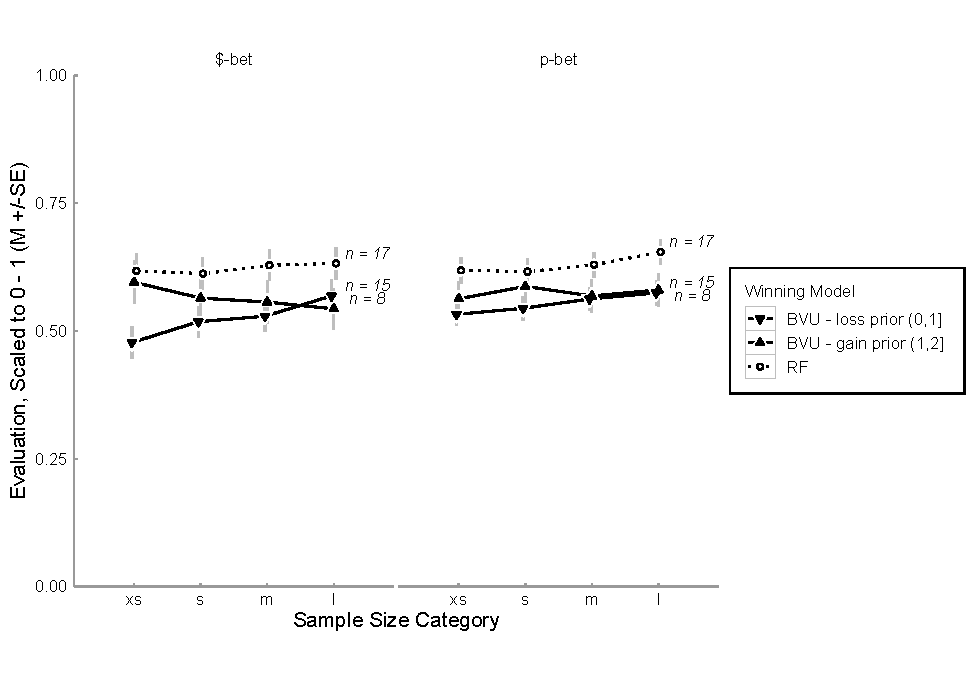
\includegraphics{../figures/qual2-1} 

}

\caption{Mean evaluation (standardized to 0 - 1) by winning model and prior beliefs of the BVU model. \textit{BVU}$=$Bayesian value updating model, \textit{RF}$=$ Relative frequency model. Error bars indicate standard errors. \textit{\$-bet}: low-probability high-outcome gambles, \textit{p-bet}: high-probability low-outcome gambles. Sample sizes (xs, x, m, l), see Table \ref{tab:Lotteries}. \textit{n=16, 13, 6} denotes the number of participants best-described by the respective models.}\label{fig:qual2}
\end{figure}

\subsubsection{Effect of gamble type and sampling order}

In line with Study 1, the mean and median ratings in Table
\ref{tab:means_study2} show that \$-bets are evaluated higher than
p-bets, although he gamble types had the same expected value
(BF\textsubscript{10} \textgreater 1,000). Again, we did not find
evidence for any recency or primacy effects.
\(\mathrm{M}\textsubscript{0}\), which predicts valuations as a function
of the factor gamble (1--6), was slightly preferred over models that
also include the mean of the first half of the observed samples
(\(\mathrm{M}\textsubscript{1}\)) or the mean of the second half of the
observed samples (\(\mathrm{M}\textsubscript{2}\)) as predictors
(\(BF\textsubscript{01} = 3.4\), \(BF\textsubscript{02} = 1.9\)).

\subsubsection{Confidence ratings}

Participants' mean confidence ratings of their valuations from
experience in the extra small, small, medium, and large sample-size
categories were (\(M (SD)\)) equal to 4.01 (\(1.23\)), 4.09, (\(1.14\)),
4.04 (\(1.19)\), and 4.16 (\(1.19\)). for sample size categories xs, s,
m, and l, respectively. Sample size did not influence participants'
confidence systematically: \(\mathrm{M}\textsubscript{0}\), which
predicts confidence rating as a function of a random participant effect,
was strongly preferred over \(\mathrm{M}\textsubscript{1}\), which in
addition includes the sample-size category as a predictor
(\(BF\textsubscript{01} = 737\)).

\added[id=jj]{The Bayesian cognitive strategy predicts that confidence increases with higher sample sizes; the relative frequency model predicts that sample size has no influence on confidence. To test this, the confidence data was analyzed separately by best-fitting cognitive model (Bayesian-type learners or relative-frequency-type learners). Contrary to the expectations, the Bayesian learners' confidence did not increase with higher sample sizes ($M=3.94, 4.01, 3.96, 4.12$ for sample sizes xs, s, m, l, respectively. Respective \textit{SD}s $= 1.29, 1.18, 1.20, 1.25$). A linear model\footnote{with by-participant random intercept and the predictors effect-coded.} of the confidence ratings, which excluded sample size as predictor, was preferred over a model including sample size (BF\textsubscript{excl,incl} $= 100$). Similarly, the confidence of relative-frequency-type learners did not show an effect of sample size on confidence ratings ($M=4.11, 4.20, 4.14, 4.21$ for sample sizes xs, s, m, l, respectively; \textit{SD}s $= 1.12, 1.08, 1.17, 1.10$, respectively; BF\textsubscript{excl,incl} $= 0.70$)}.

\subsubsection{Description versus experience}

The above Table \ref{tab:means_study2} summarizes the valuations from
description; it also shows the difference between the mean valuations in
the experience and description conditions (column D--E, separately for
different sample sizes). Further, it provides the Bayes factors,
quantifying the evidence in favor of a difference between valuations
from experience and those from description.

Valuations made from description and experience differed for most of the
gambles and sample sizes (see Table \ref{tab:means_study2}, rightmost
column). In particular, participants attached a higher value to
experienced than to described \$-bets (Gambles 1--3) but attached a
higher value to described than to experienced p-bets (Gambles 4--6).
Thus, we found a D--E gap that is the opposite of the classic D--E gap
observed in choice paradigms. In our study, participants valued gambles
as if they overweighted rare events from description \textit{and}
experience. This effect was even stronger when people made valuations
from experience.

We also compared participants' confidence ratings of valuations from
experience in each sample-size category to those from description
(\(M = 4.04\), \(SD = 1.08\)). Separately for each sample-size category,
we compared \(\mathrm{M}\textsubscript{0}\), which predicts confidence
as a function of random participant effects, with
\(\mathrm{M}\textsubscript{1}\), which takes condition as an additional
fixed factor into account. The analyses suggest that participants were
slightly more confident about their ratings from experience than from
description for small (\(BF\textsubscript{10} = 2.5\)), medium
(\(BF\textsubscript{10} = 1.3\)), and large
(\(BF\textsubscript{10} = 4.8\)) sample sizes. For the extra small
sample sizes (\(BF\textsubscript{10} = 0.3\)), confidence judgments did
not differ.


\end{document}
